\paragraph{Objectives of the COORD subproject.}
%\begin{figure}
%\centering
%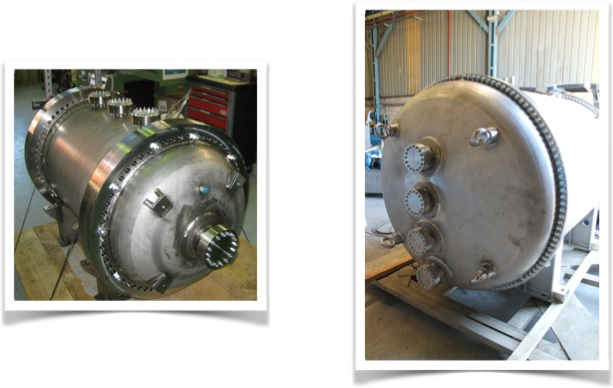
\includegraphics[height=8cm]{img/PV.jpg}
%\caption{The pressure vessel of NEW (left) and NEXT-100 (right).} \label{fig:PV}
%\end{figure}

%%%%%
\begin{figure}[t!b!]
\begin{center}
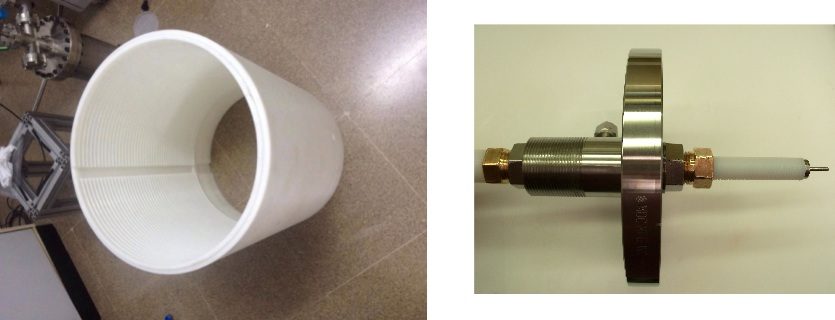
\includegraphics[width=.9\textwidth]{img/FC3.jpg}
\end{center}
\caption{Left: The NEW field cage body made of HDPE, fabricated in Spain; right: The anode HVFT manufactured in Texas.
} \label{fig:FC}
\end{figure}

%%%%%
\begin{figure}[t!b!]
\begin{center}
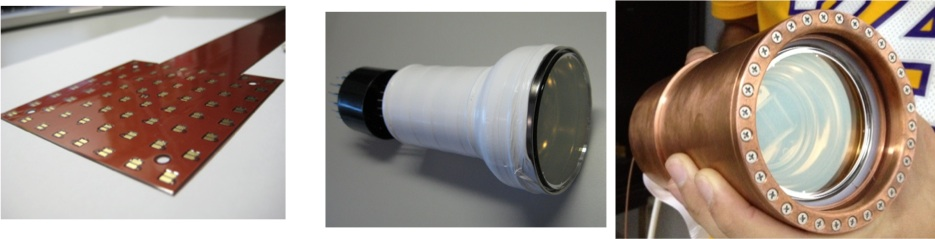
\includegraphics[width=.9\textwidth]{img/KDBandPMT.jpg}
\end{center}
\caption{Top left: the flexible Kapton Dice Board (KDB) circuit developed by NEXT for the tracking plane; mid: the R11410-10 PMT from Hamamatsu; bottom right: a PMT can prototype.} \label{fig:sensors}
\end{figure}

The specific objectives of the COORD subproject are:

\begin{enumerate}
\item {\bf Construction of NEW}, foreseen to be completed in Q2'15, and involving the construction of the NEW pressure vessel, field cage, energy plane, tracking plane.

\item {\bf Commissioning of NEW and evaluation of performance}. The NEW detector will be brought online in Q2'15, and extensive system testing will be performed to certify safe and stable operation (no leaks, no sparks), as well as testing and integration of all the subsystems. We expect to complete commissioning in Q3'15.
During Q4'15, we will evaluate the performance of the detector. Such evaluation will allow us to correct for design problems (if they arise) or to introduce improvements in the engineering if needed. We will also assess the overall radioactive budget of the detector, to ensure the absence of ``hot spots'' (excess of radioactivity introduced accidentally in the detector). 

\item {\bf NEW physics run}. During 2016, we will operate continuously the NEW detector at the LSC. The physics runs of NEW has several goals: a) measurement, using radioactive sources, of the energy resolution as a function of the energy, and in particular at \Qbb (CALREC subproject) ; b) measurement, using radioactive sources, of single (``background'') electrons, as well as ``double electrons'' (produced by the double escape peak of Tl-208, and used to characterise the signal) (COORD and CALREC); c) measurement of the standard mode \bbtnu; and d) a full measurement of the spectrum, after selection cuts, thus quantifying, from the data themselves, the background model (collaboration wide studies). 
%

\item {\bf Construction of NEXT-100}. The fabrication of NEXT-100 will proceed through 2016, although some parts (such as the pressure vessel) have already been built. The construction will take 12 months. 

\item {\bf Commissioning of NEXT-100}. The commissioning of NEXT-100 will benefit from the experience gained commissioning and operating NEW. We consider feasible to commission the detector during the first 2 quarters of 2017, but our project management plan allows for two extra quarters. The main reason is to guarantee enough time to run with normal xenon before circulating the precious enriched xenon in the gas system and the detector. Notice that the detector can be fully calibrated, and the backgrounds can be characterised with normal xenon.  

\item {\bf Physics run of NEXT-100}. The physics run may start in the third quarter of 2017, but the project plan foresees the first quarter of 2018. The calibration procedures are identical to those developed for NEW. After one year of run, NEXT-100 should reach the sensitivity of the current leading experiments. We currently foresee to run for three years (2018 to 2020), achieving a sensitivity to \mbb\ that makes a discovery possible if NME are sufficiently large and the neutrino is a Majorana particle. 

\end{enumerate}
